\chapter{Implémentation}
\label{chap:impl}

\section{Technologies utilisées}

\subsection{Backend}

Le backend est implémenté en \textbf{PHP} avec le framework \textbf{Laravel} \cite{laraveldoc}. Les routes REST sont définies dans \texttt{routes/api.php} et regroupées par préfixes (\texttt{/api/client}, \texttt{/api/employee}, \texttt{/api/admin}, \texttt{/api/public}). La persistance utilise \textbf{Eloquent ORM} sur \textbf{PostgreSQL} \cite{postgresdoc}. Les règles de validation métier sont exprimées dans des classes \texttt{Form Request} lorsque pertinent. Les envois d'e-mails passent par le sous-système \texttt{Mail} de Laravel et, selon la configuration, par un connecteur \textbf{EmailJS} côté application pour certaines notifications.

\subsection{Authentification et sécurité API}

L'authentification du \emph{single page application} repose sur \textbf{Laravel Sanctum} en mode \emph{stateful} \cite{sanctumdoc} : après récupération du cookie CSRF via \texttt{GET /sanctum/csrf-cookie}, le client envoie les requêtes avec \texttt{withCredentials: true} et l'en-tête \texttt{X-XSRF-TOKEN} synchronisé sur le cookie \texttt{XSRF-TOKEN}. La connexion utilise \texttt{Auth::attempt} et régénère la session ; les routes protégées passent par le middleware \texttt{auth:sanctum}. Les autorisations fines combinent middlewares \texttt{role:...} et \texttt{perm:...} alignés sur les tables \texttt{roles}, \texttt{permissions} et la table pivot \texttt{role\_user}.

\subsection{Frontend}

Le frontend est développé en \textbf{React} (JavaScript) avec \textbf{Vite} comme outil de build \cite{reactdoc,vitedoc}. Le routage est assuré par \textbf{React Router v6}. Les appels HTTP utilisent \textbf{Axios} via un client central (\texttt{axiosClient}) configuré avec \texttt{withCredentials} et la protection CSRF Sanctum. L'état d'authentification est géré par un \texttt{AuthContext} (profil utilisateur via \texttt{GET /api/me}).

\newpage
\subsection{Base de données et outillage}

PostgreSQL sert de SGBD principal \cite{postgresdoc}. Le schéma est versionné par les \textbf{migrations Laravel} (\texttt{database/migrations}). Le dépôt du stage contient les dossiers \texttt{03\_Backend\_Laravel/eservices-api} et \texttt{04\_Frontend\_React/eservices-front}.

\subsection{Conteneurisation et exécution locale}

L'API et le frontend peuvent être lancés en développement sur la machine hôte (serveur PHP Artisan, serveur Vite). Une conteneurisation type Docker reste possible pour la démonstration (API, frontend, PostgreSQL, volumes pour pièces jointes) \cite{dockerdoc,twelvefactor}.

\section{Structure du projet}

\subsection{Arborescence backend (logique Laravel)}

Le backend suit les conventions Laravel : \texttt{app/Http/Controllers} (contrôleurs par domaine : \texttt{Admin}, \texttt{Client}, \texttt{Employee}, \texttt{Staff}, \texttt{Public}), \texttt{app/Models} (notamment \texttt{User}, \texttt{Service}, \texttt{ServiceField}, \texttt{Request}, \texttt{RequestHistory}, \texttt{RequestDocument}, \texttt{RequestComment}, \texttt{Agency}, \texttt{Role}), \texttt{app/Services} (ex. \texttt{RequestNotificationService}), \texttt{app/Mail}, \texttt{routes/api.php}, \texttt{database/migrations}.

\subsection{Arborescence frontend (logique React)}

Le frontend est organisé en \texttt{src/pages} (portails \texttt{client}, \texttt{admin}, \texttt{employee}, pages publiques \texttt{login}, \texttt{register}, formulaire public \texttt{/demande/:serviceId}), \texttt{src/components}, \texttt{src/api}, \texttt{src/auth}, \texttt{src/routes} (garde d'accès par rôle).

\section{Fonctionnalités implémentées (alignement code)}

\subsection{Rôles et permissions}

Les rôles métier sont stockés en base (\texttt{roles}, attribut \texttt{name}) et associés aux utilisateurs via \texttt{role\_user}. Le jeu effectivement utilisé par l'application inclut notamment : \texttt{admin} (accès complet back-office), \texttt{client} (portail usager), \texttt{agent} et \texttt{responsable} (parcours staff : services pour le responsable, demandes pour l'agent et le responsable selon les routes), \texttt{director} et \texttt{reception} (portail \texttt{/employee} pour le suivi opérationnel). Les permissions nommées (\texttt{manage\_services}, \texttt{view\_all\_requests}, etc.) sont mappées dans le seeder et exploitées par middleware.

\subsection{Conception dynamique des services}

Un service est rattaché à une \textbf{agence} (\texttt{agency\_id}), possède des métadonnées (nom, description, textes d'aide, critères, durée estimée, activation) et des dates optionnelles de \textbf{publication} et de \textbf{clôture des dépôts} (\texttt{published\_at}, \texttt{request\_deadline\_at}). Les champs de formulaire sont des enregistrements \texttt{service\_fields} (clé, libellé, type, obligatoire, ordre, placeholder, options JSON). L'API admin expose le CRUD champs et le réordonnancement.

\subsection{Gestion des services et des demandes}

Le front admin propose la gestion de tableaux de services et de demandes branchés sur \texttt{/api/admin/services} et \texttt{/api/admin/requests} (filtres, pagination, actions : affectation, changement d'état, commentaires, pièces jointes, marquage « vu », activation/désactivation). Le portail client consomme \texttt{/api/client/requests} et le catalogue public \texttt{/api/services}.

\subsection{Demande publique sans compte}

Une route frontend \texttt{/demande/:serviceId} et des endpoints \texttt{/api/public/requests} permettent de créer et suivre une demande avec \textbf{jeton public} retourné à la création, sans authentification Sanctum.

\subsection{Notifications e-mail}

Le service \texttt{RequestNotificationService} centralise une partie des notifications : libellés d'état en français, envoi via \texttt{Mail::} (messages \texttt{RequestActivityMail}, \texttt{ServicePublishedClientMail}, etc.) et mécanisme EmailJS configurable. Une commande planifiée balaie les services à notifier après publication.

\subsection{Agences et employés}

Les agences sont gérées via \texttt{AgencyController} (CRUD côté admin). Les utilisateurs (employés) sont administrés via \texttt{UserAdminController} avec filtrage par rôle et rattachement d'agence.

\subsection{Paramètres utilisateur}

La mise à jour du profil authentifié passe par \texttt{PUT /api/me} (\texttt{ProfileController}) et, pour le client, \texttt{PUT /api/client/profile}.

```latex
\section{Interfaces graphiques implémentées}

Afin de compléter la description fonctionnelle présentée précédemment, cette section expose les principales interfaces graphiques développées au sein de la plateforme E-Services \#ADD. Les captures d'écran permettent d'illustrer concrètement les fonctionnalités implémentées, l'organisation du back-office et les interactions offertes aux différents profils d'utilisateurs.

\subsection{Parcours d'authentification et gestion des accès}

L'authentification constitue la première étape d'interaction entre l'utilisateur et la plateforme. Elle permet de sécuriser l'accès aux différents espaces selon le rôle attribué à chaque utilisateur.

\subsubsection{Connexion}

\begin{figure}[H]
\centering
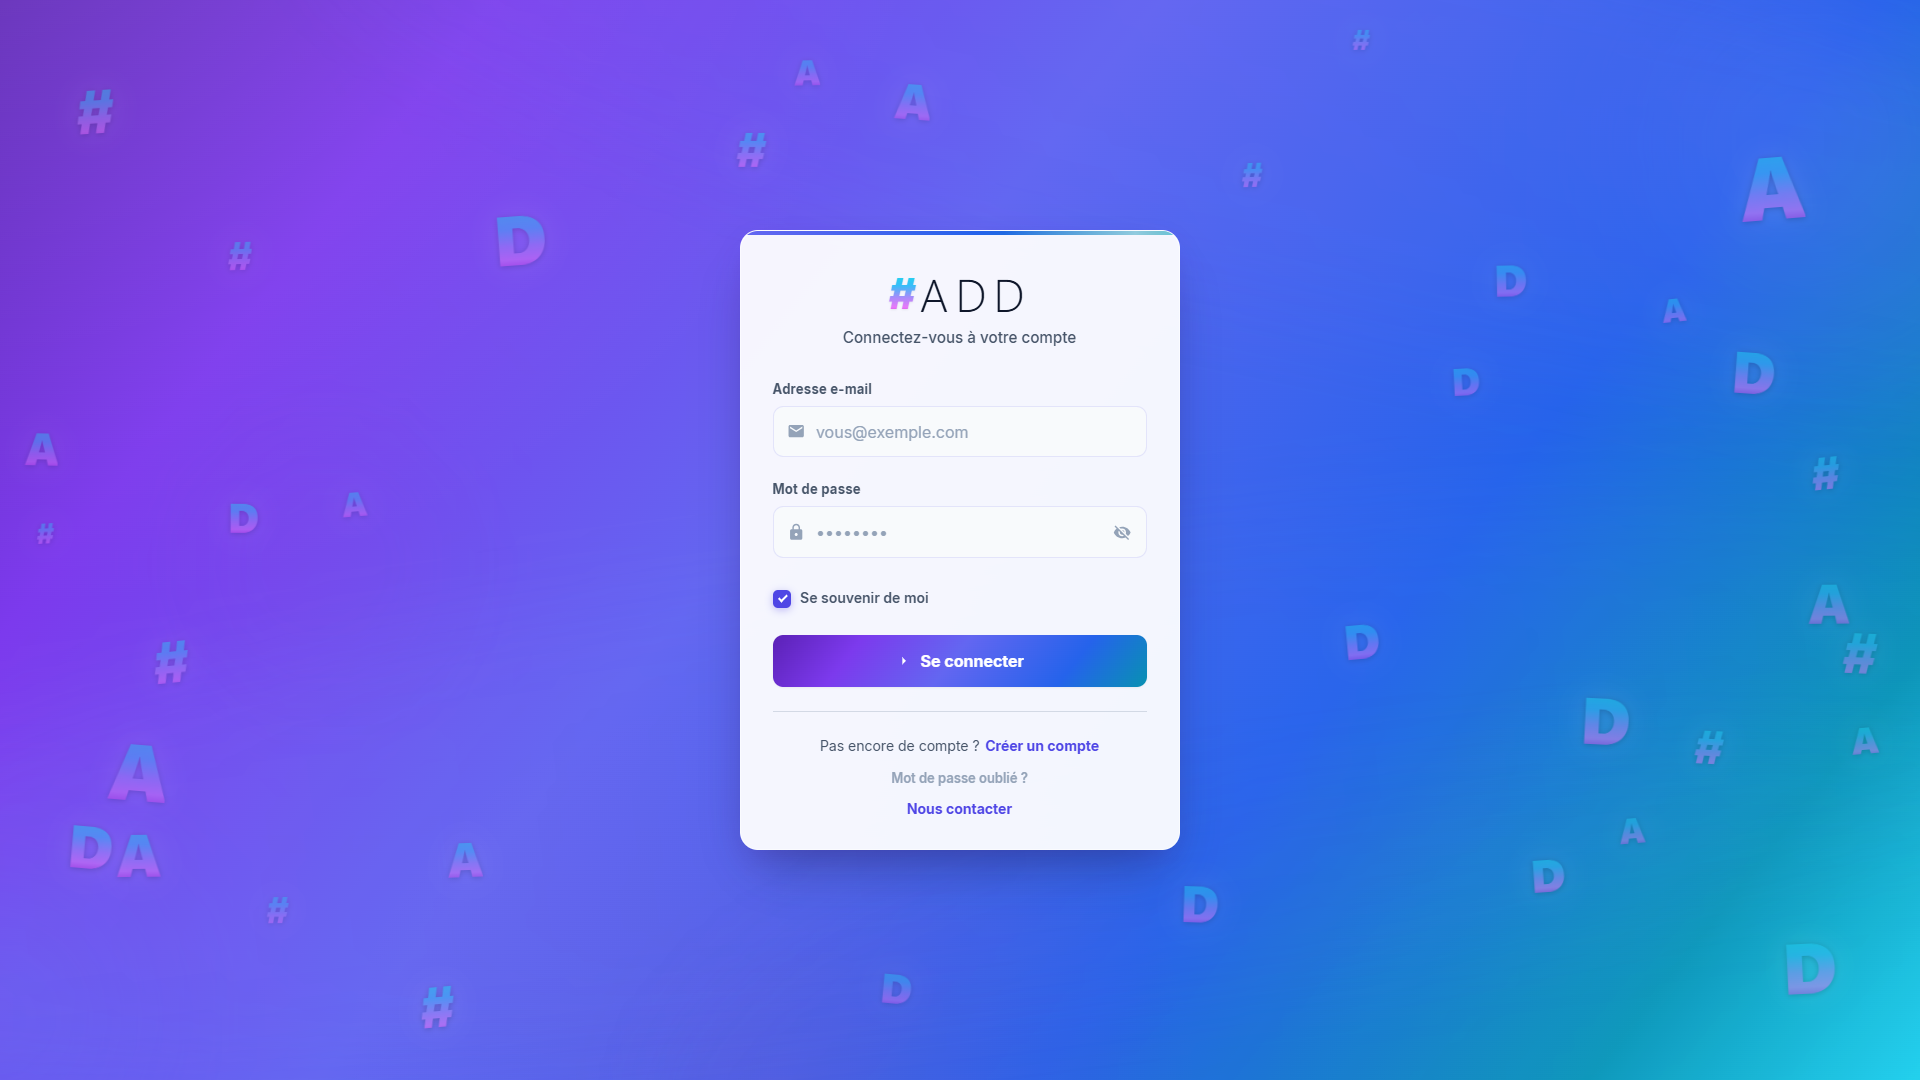
\includegraphics[width=0.9\textwidth]{auth-login.png}
\caption{Écran de connexion par adresse e-mail et mot de passe.}
\label{fig:auth-login}
\end{figure}

La figure~\ref{fig:auth-login} présente l'écran de connexion de la plateforme E-Services. Cette interface permet à l'utilisateur de saisir son adresse e-mail et son mot de passe afin d'accéder aux fonctionnalités correspondant à son rôle. Elle constitue le point d'entrée principal vers les espaces sécurisés de l'application et s'appuie sur le mécanisme d'authentification Laravel Sanctum décrit précédemment.

\subsubsection{Inscription}

\begin{figure}[H]
\centering
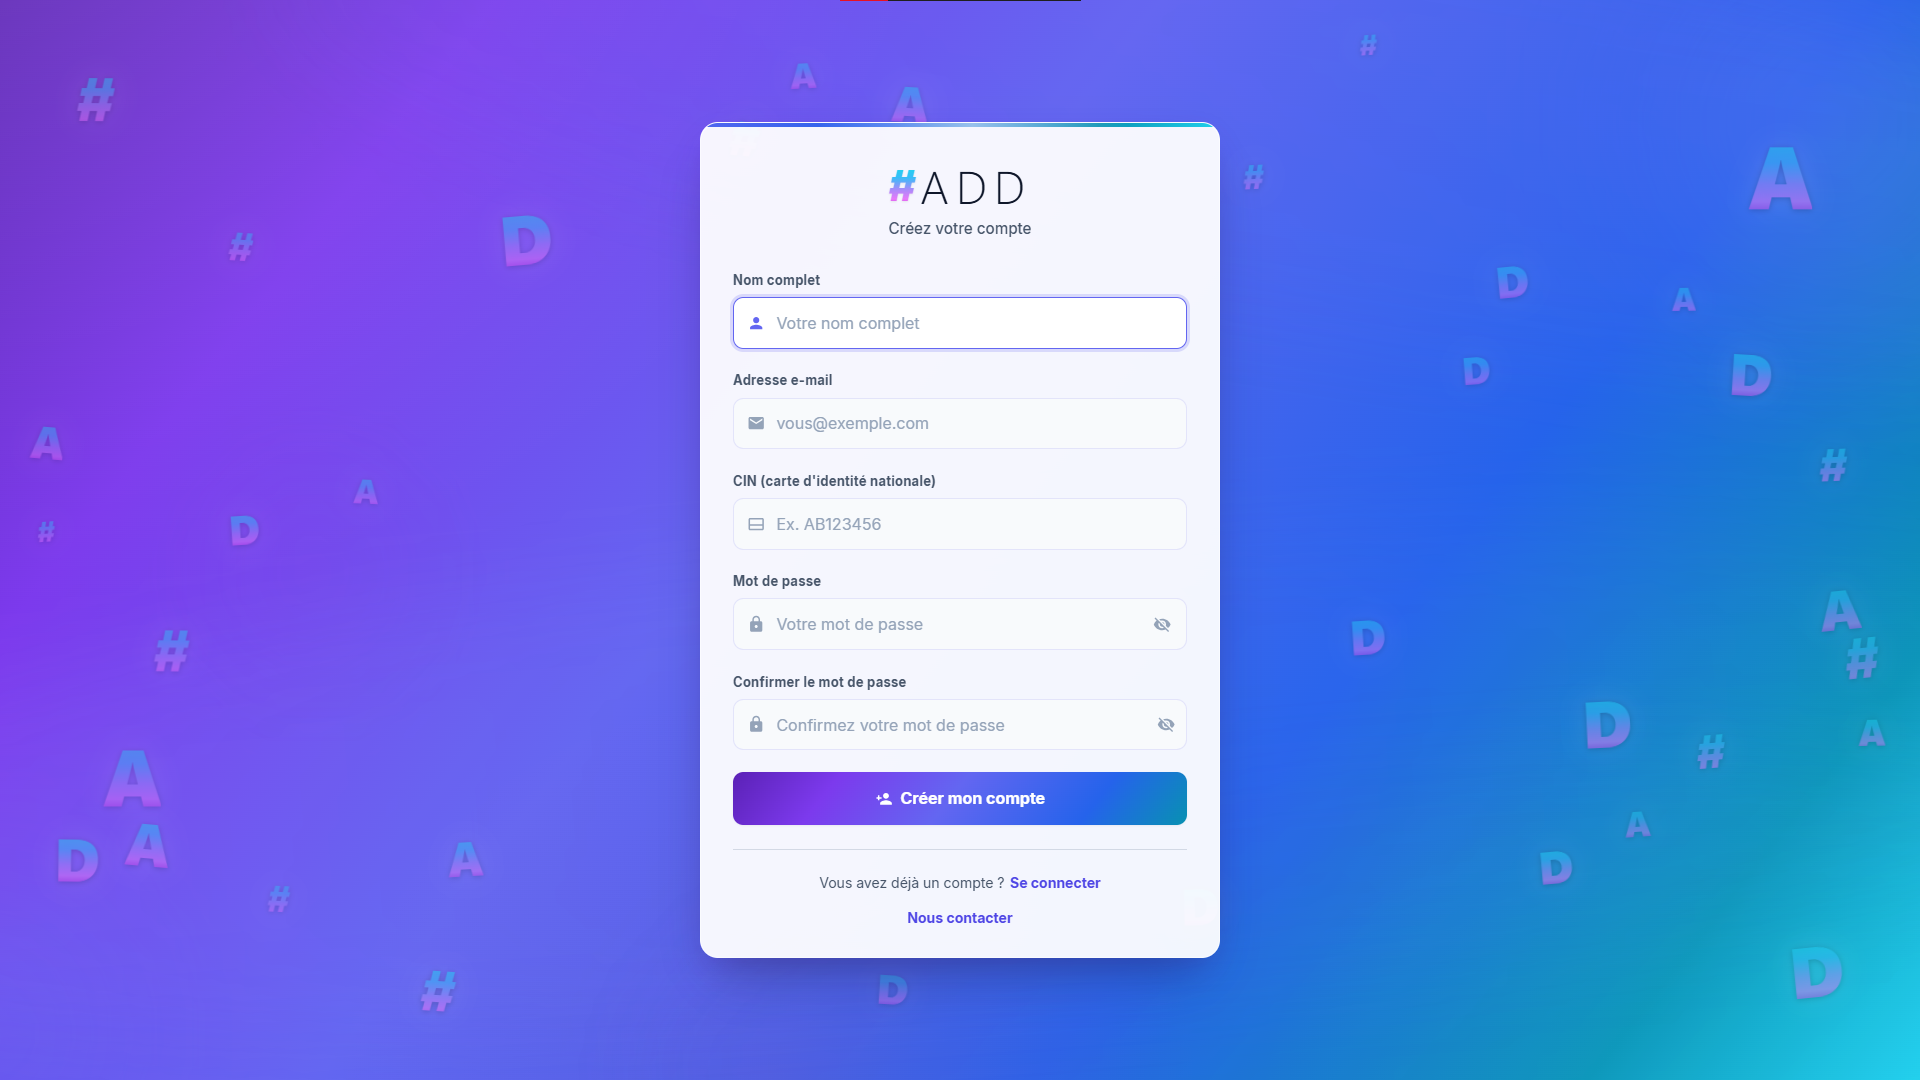
\includegraphics[width=0.9\textwidth]{auth-register.png}
\caption{Formulaire d'inscription d'un nouvel usager.}
\label{fig:auth-register}
\end{figure}

La figure~\ref{fig:auth-register} illustre le formulaire d'inscription destiné aux nouveaux usagers. Cette interface permet de collecter les informations nécessaires à la création d'un compte, notamment le nom complet, l'adresse e-mail, le CIN et le mot de passe. Les données saisies sont validées avant leur enregistrement afin de garantir leur cohérence et leur intégrité.

\newpage
\subsubsection{Récupération du mot de passe}

\begin{figure}[H]
\centering
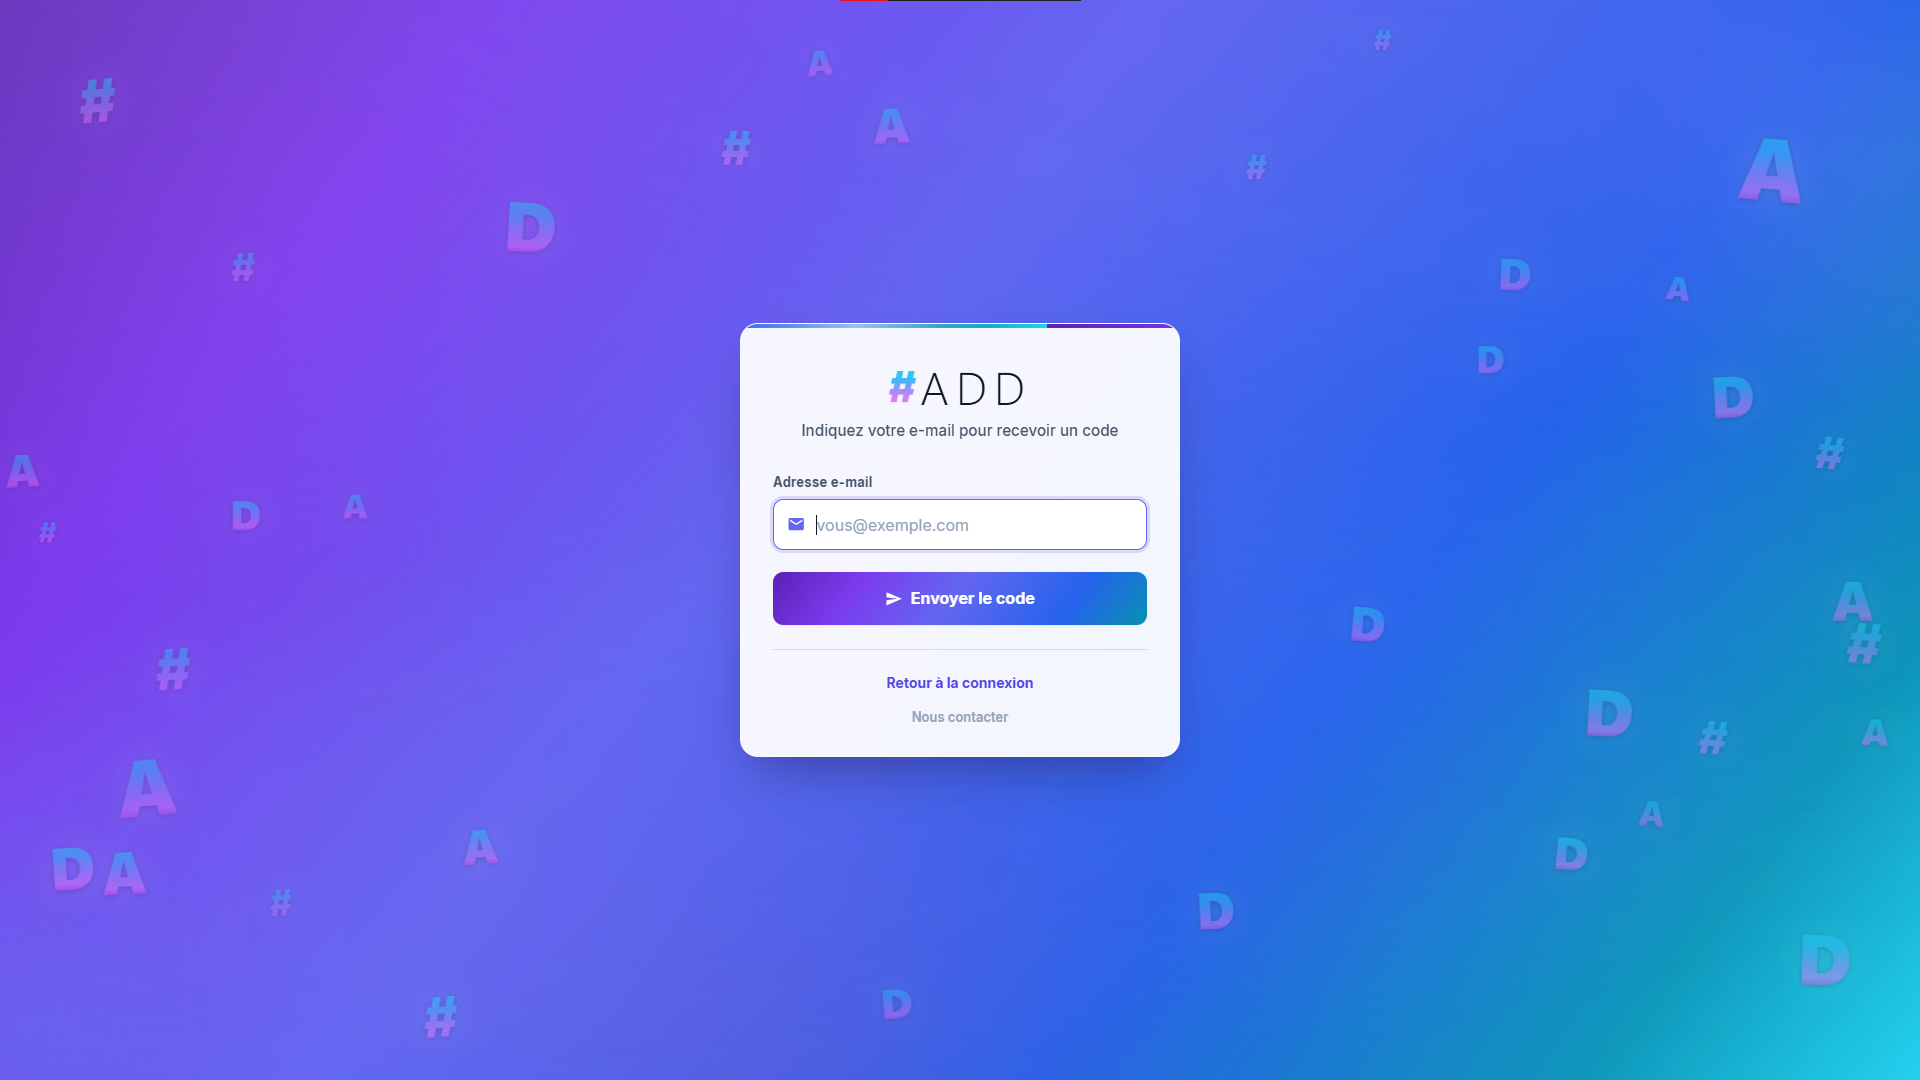
\includegraphics[width=0.9\textwidth]{auth-forgot-password.png}
\caption{Première étape de récupération du mot de passe oublié.}
\label{fig:auth-forgot-password}
\end{figure}

La figure~\ref{fig:auth-forgot-password} présente la première étape de récupération du mot de passe. L'utilisateur renseigne son adresse e-mail afin de recevoir un code de vérification. Cette fonctionnalité améliore l'autonomie de l'utilisateur tout en maintenant un niveau de sécurité adapté à la gestion des accès.
\newpage
\begin{figure}[H]
\centering
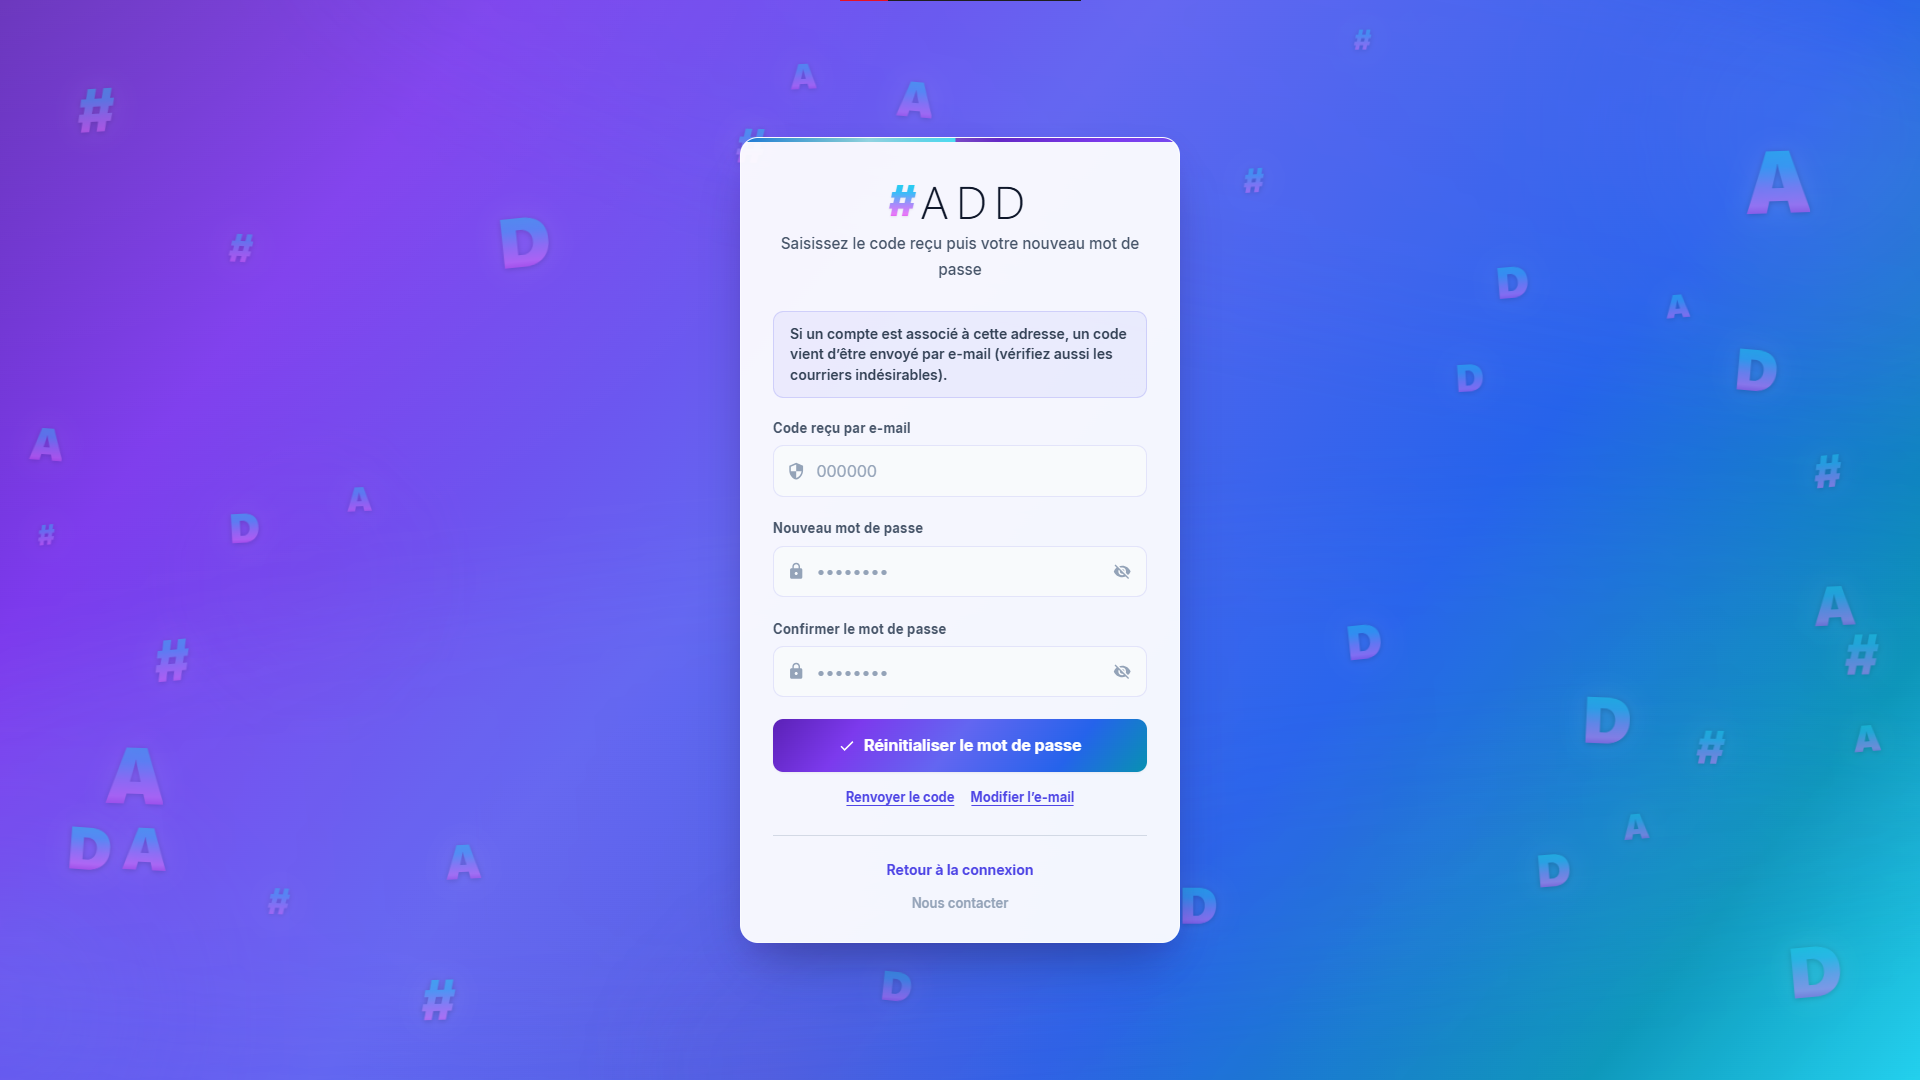
\includegraphics[width=0.9\textwidth]{auth-reset-password.png}
\caption{Seconde étape de réinitialisation du mot de passe.}
\label{fig:auth-reset-password}
\end{figure}

La figure~\ref{fig:auth-reset-password} montre la seconde étape du processus de réinitialisation. Après réception du code de vérification par e-mail, l'utilisateur peut définir un nouveau mot de passe. Le système vérifie la validité du code ainsi que la conformité des informations saisies avant la mise à jour des données d'authentification.

\newpage
\subsection{Interface générale du portail administrateur}

Le portail administrateur repose sur une interface structurée autour d'un menu latéral, d'un en-tête, d'une identité visuelle et d'un système de notifications. Ces éléments assurent une navigation claire entre les différents modules du back-office.

\subsubsection{Menu latéral}

\begin{figure}[H]
\centering
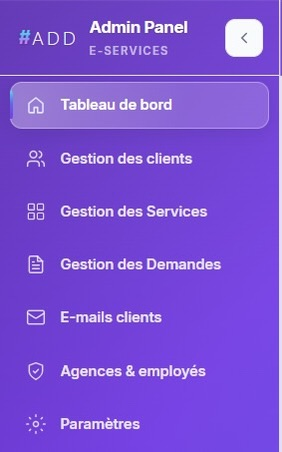
\includegraphics[width=0.45\textwidth]{admin-sidebar-expanded.jpeg}
\caption{Menu latéral du portail administrateur en mode développé.}
\label{fig:admin-sidebar-expanded}
\end{figure}

La figure~\ref{fig:admin-sidebar-expanded} présente le menu latéral du portail administrateur en mode développé. Il regroupe les principaux modules de gestion, notamment le tableau de bord, les clients, les services, les demandes, les e-mails, les agences, les employés et les paramètres.
\newpage
\subsubsection{En-tête et identité visuelle}

\begin{figure}[H]
\centering

\includegraphics[width=1\textwidth]{admin-header.png}
\caption{En-tête du portail administrateur avec titre, notifications et profil connecté.}
\label{fig:admin-header}
\end{figure}

La figure~\ref{fig:admin-header} présente l'en-tête du portail administrateur. Il affiche le titre de la page courante, l'accès aux notifications et un message d'accueil personnalisé indiquant l'utilisateur connecté.

\begin{figure}[H]
\centering

\includegraphics[width=1\textwidth]{admin-brand-mark.png}
\caption{Élément de marque \#ADD intégré dans l'en-tête.}
\label{fig:admin-brand-mark}
\end{figure}

La figure~\ref{fig:admin-brand-mark} met en évidence l'identité visuelle de la plateforme. L'intégration du logo \#ADD dans l'en-tête permet de renforcer la cohérence graphique de l'application et d'assurer une continuité visuelle entre les différents modules.

\newpage
\subsection{Tableau de bord administratif}

Le tableau de bord administratif constitue l'écran principal de supervision de la plateforme. Il offre à l'administrateur une vision globale sur les entités gérées, les demandes déposées et l'état général de l'activité.

\begin{figure}[H]
\centering
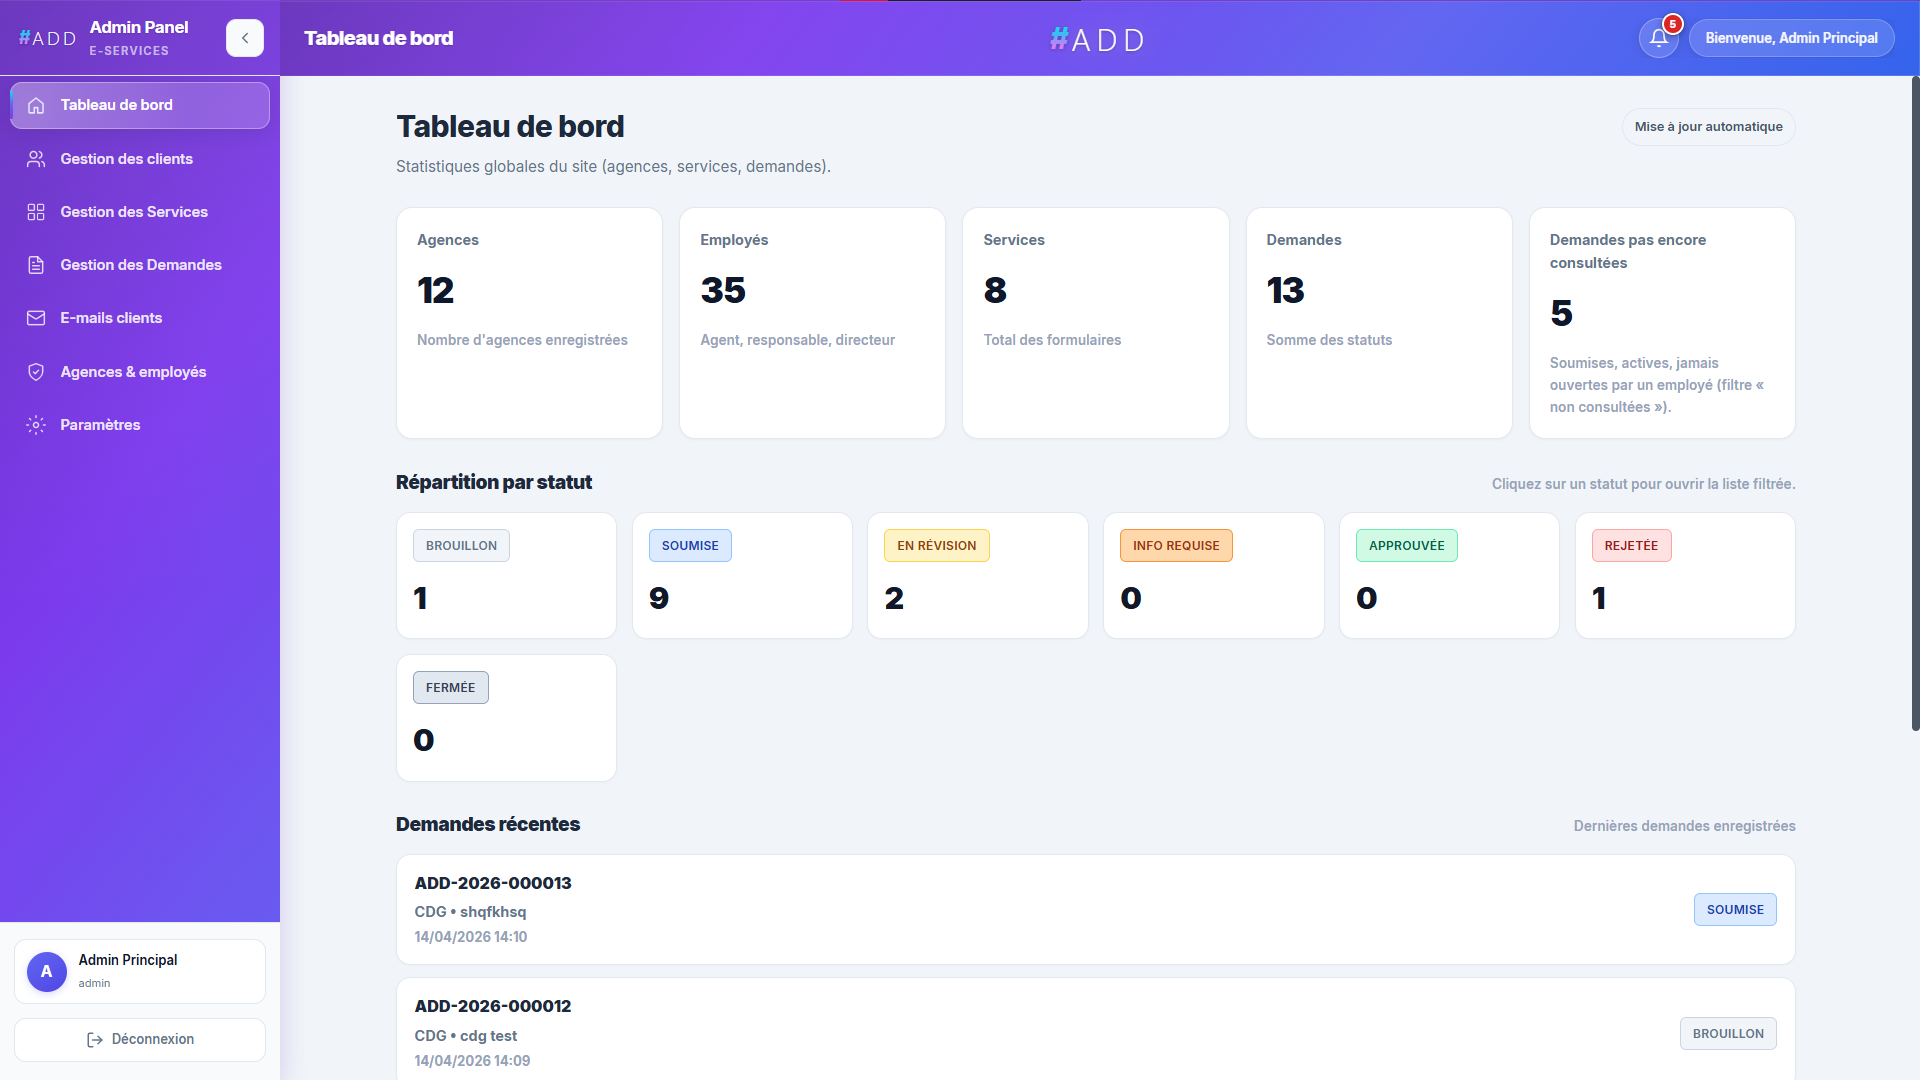
\includegraphics[width=0.95\textwidth]{admin-dashboard-top.png}
\caption{Tableau de bord administrateur avec indicateurs globaux et répartition des demandes par statut.}
\label{fig:admin-dashboard-top}
\end{figure}

La figure~\ref{fig:admin-dashboard-top} présente la partie supérieure du tableau de bord administrateur. Les cartes de synthèse affichent les principaux indicateurs du système, notamment le nombre d'agences, d'employés, de services, de demandes et de demandes non encore consultées. La répartition par statut permet de visualiser l'état d'avancement des dossiers selon le workflow implémenté.

\begin{figure}[H]
\centering
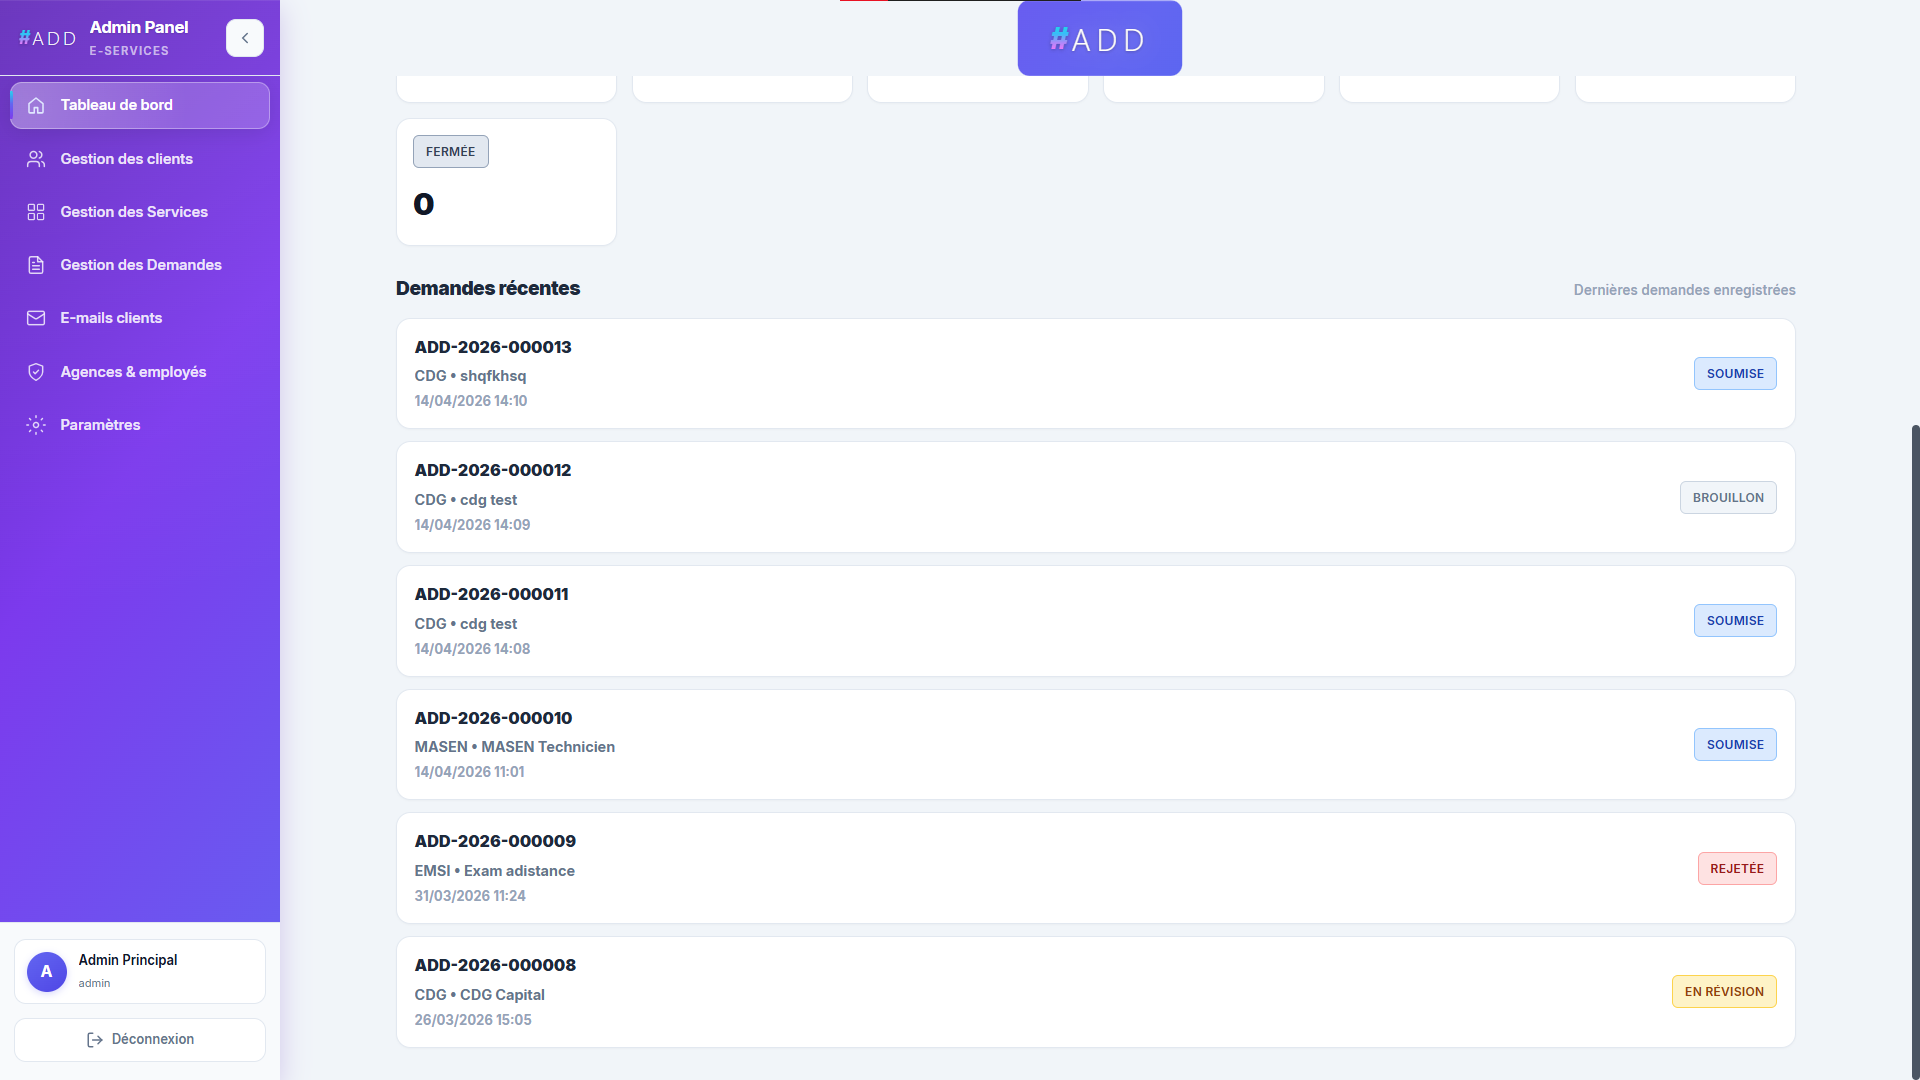
\includegraphics[width=0.95\textwidth]{admin-dashboard-buttom.png}
\caption{Liste des demandes récentes affichée dans le tableau de bord.}
\label{fig:admin-dashboard-buttom}
\end{figure}

La figure~\ref{fig:admin-dashboard-bottom} complète le tableau de bord en présentant les demandes les plus récentes. Chaque ligne affiche la référence métier, l'entité concernée, la date et l'état courant du dossier. Cette vue facilite le suivi quotidien de l'activité et permet d'identifier rapidement les demandes nécessitant une intervention.

\newpage
\subsection{Gestion des services}

Le module de gestion des services permet à l'administrateur de créer, modifier, consulter et organiser les services proposés par les agences. Il constitue un élément central de la plateforme, car il conditionne les formulaires disponibles pour les usagers.

\begin{figure}[H]
\centering
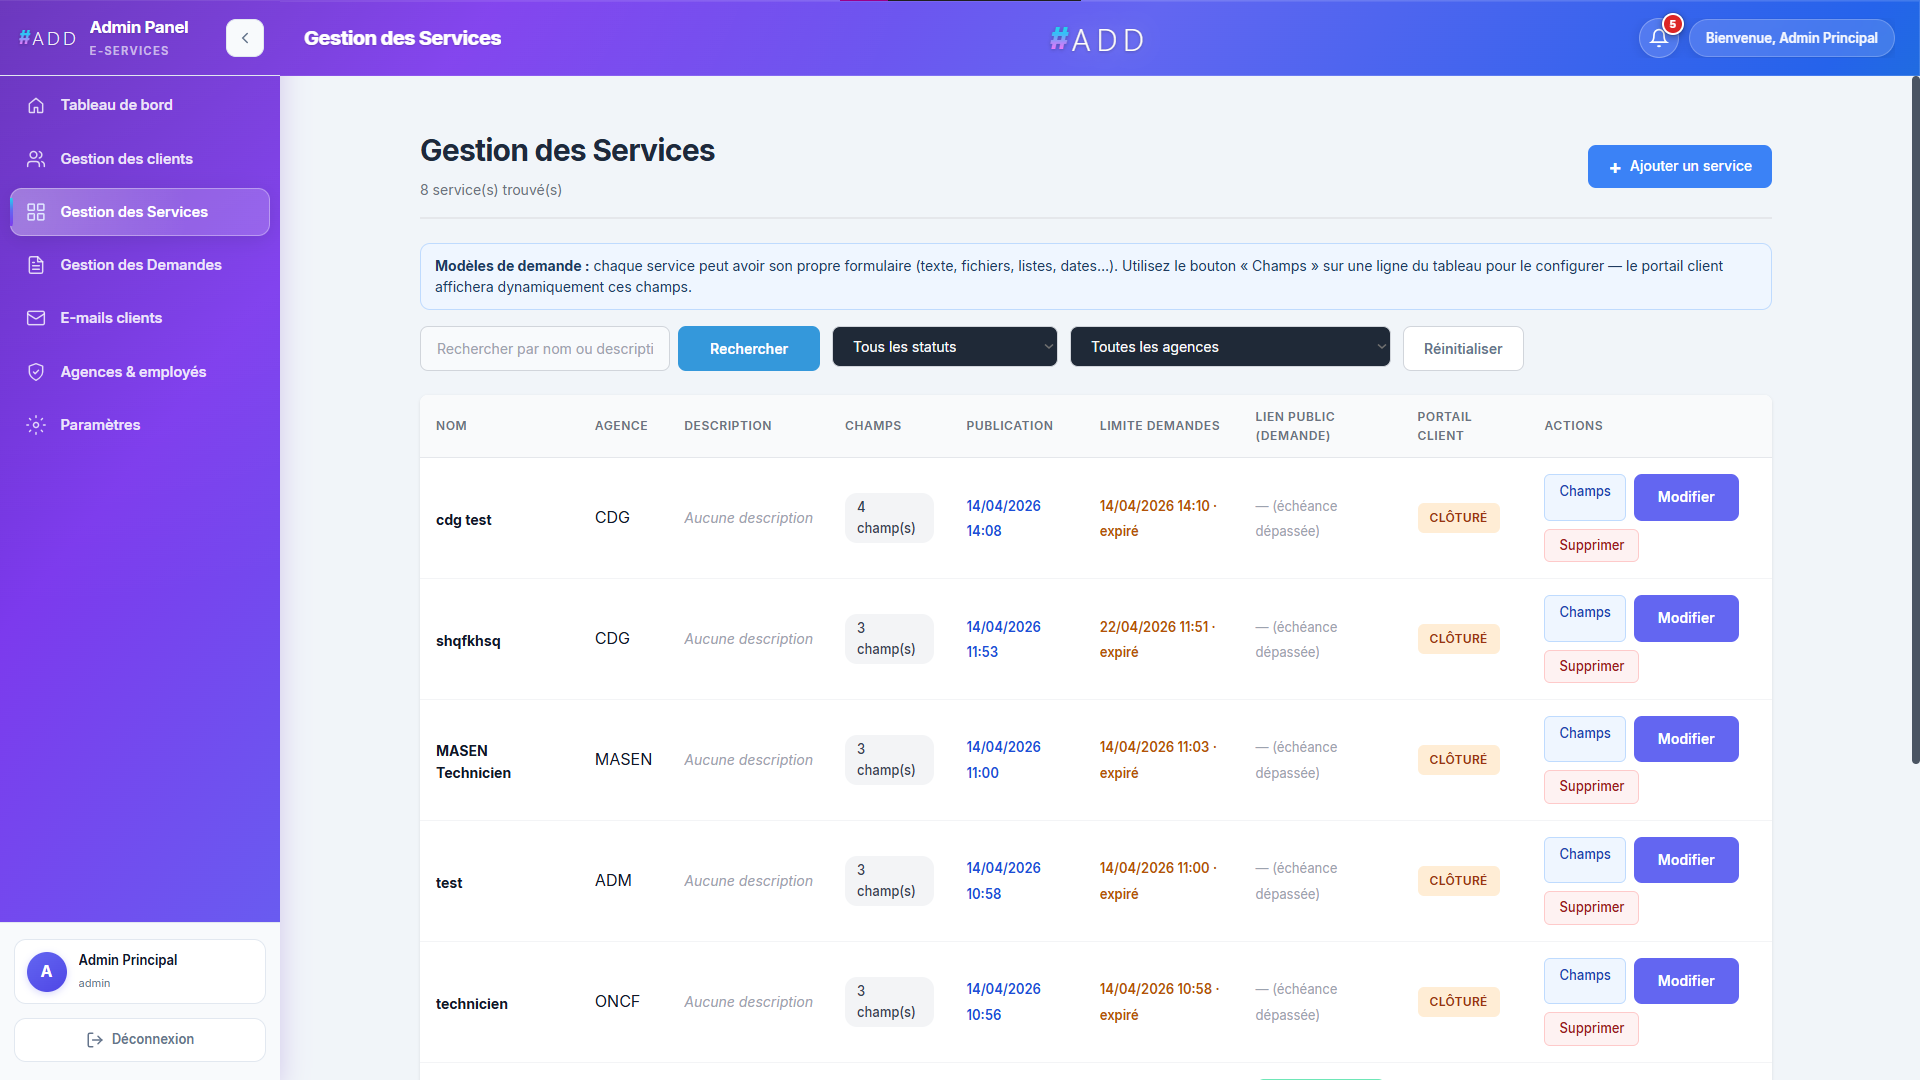
\includegraphics[width=0.95\textwidth]{admin-services-list.png}
\caption{Interface de consultation de la liste des services.}
\label{fig:admin-services-list}
\end{figure}

La figure~\ref{fig:admin-services-list} présente la liste des services disponibles dans la plateforme. Cette interface permet à l'administrateur de consulter les services existants, leurs informations principales et les actions de gestion associées.

\begin{figure}[H]
\centering
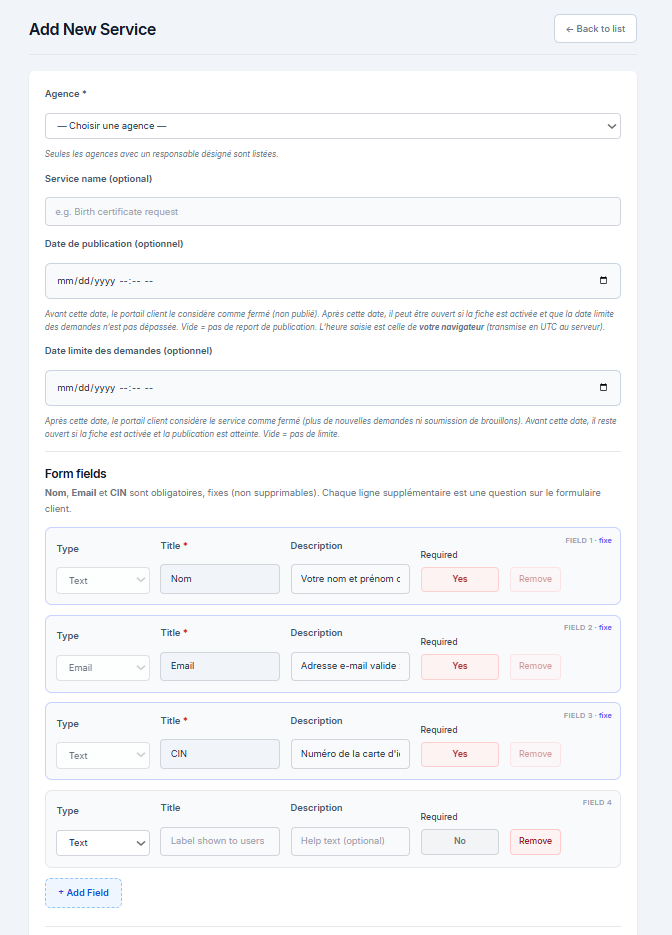
\includegraphics[width=0.95\textwidth]{admin-service-add.png}
\caption{Interface d'ajout d'un nouveau service.}
\label{fig:admin-service-add}
\end{figure}

La figure~\ref{fig:admin-service-add} illustre le formulaire d'ajout d'un nouveau service. Cette interface permet de renseigner les informations nécessaires à la publication du service et à la configuration de ses champs dynamiques.

\newpage
\subsection{Gestion des demandes}

Le module de gestion des demandes permet le suivi, l'affectation et le changement d'état des dossiers déposés par les usagers. Il assure la traçabilité du traitement et facilite la coordination entre les différents profils du back-office.

\begin{figure}[H]
\centering
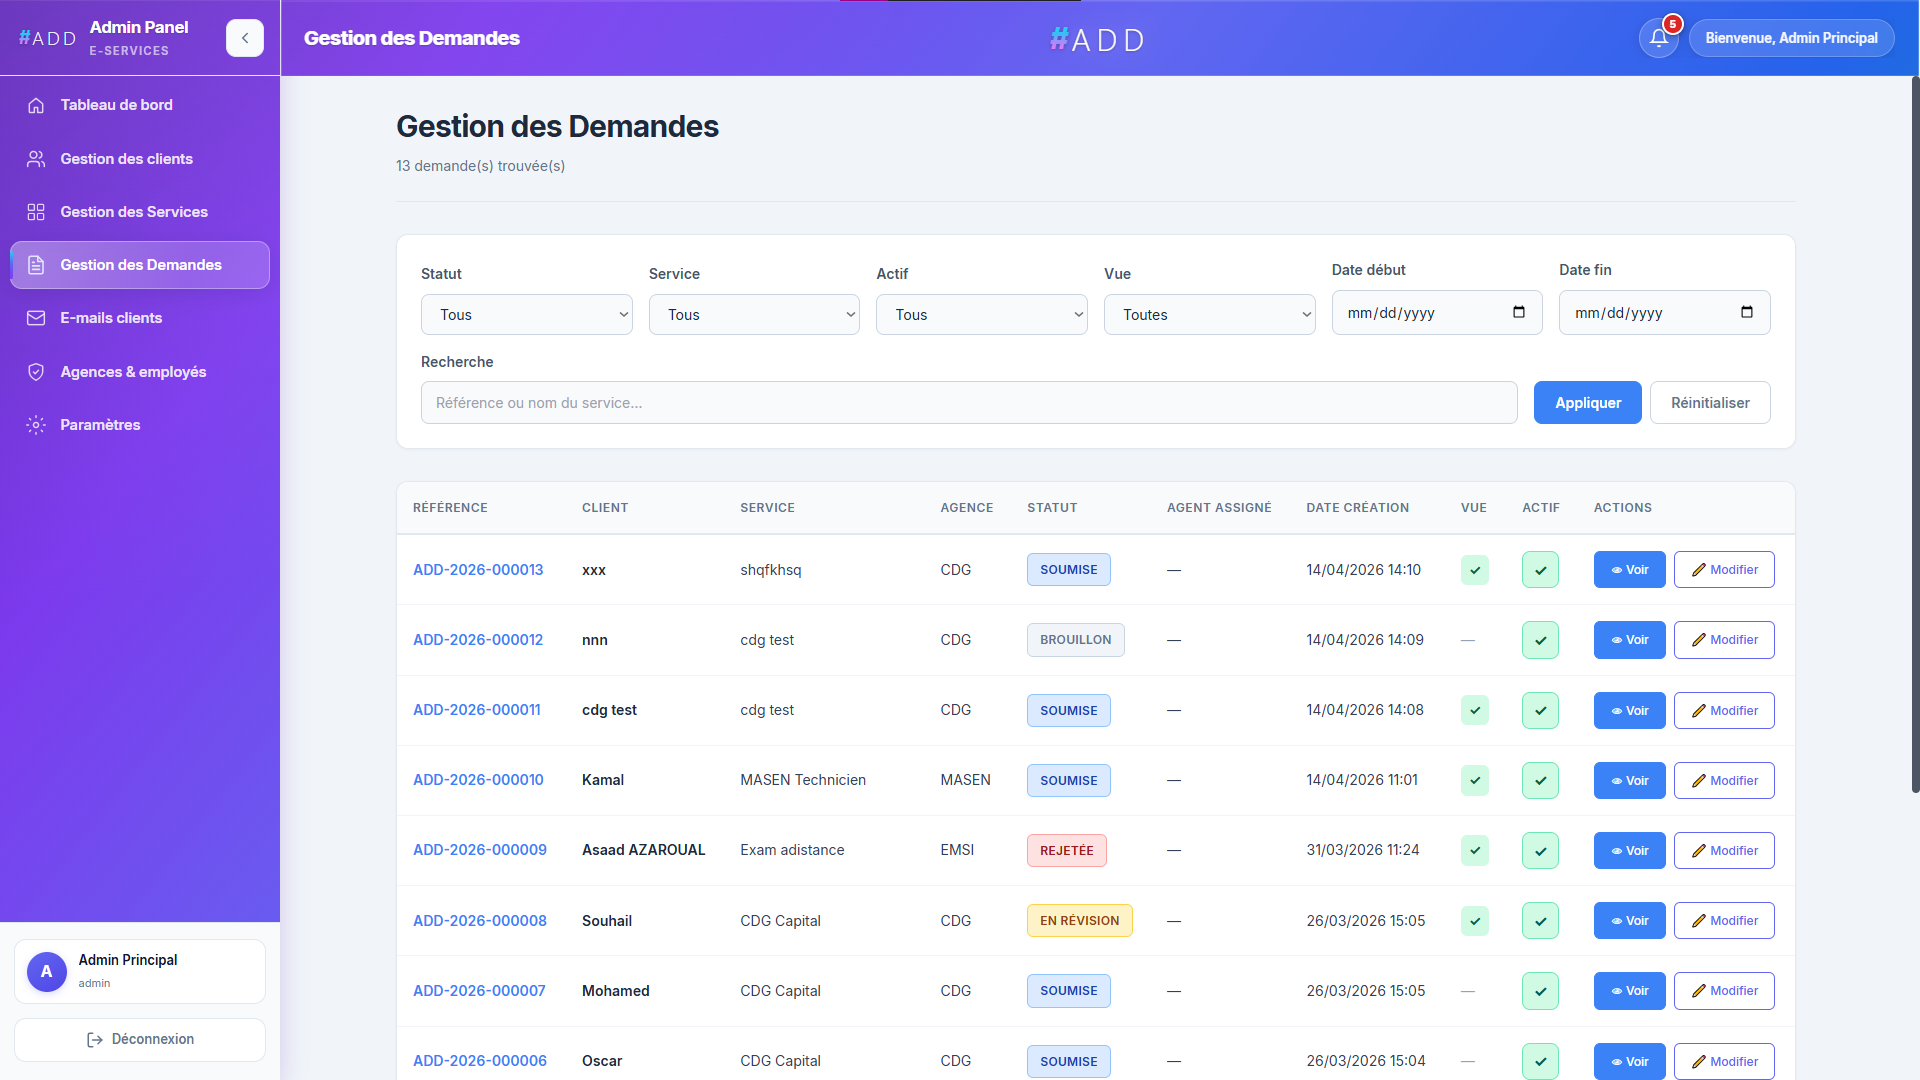
\includegraphics[width=0.95\textwidth]{admin-requests-list.png}
\caption{Interface de gestion et de suivi des demandes déposées.}
\label{fig:admin-requests-list}
\end{figure}

La figure~\ref{fig:admin-requests-list} présente la liste des demandes enregistrées dans le système. Elle permet de consulter les informations principales de chaque dossier, telles que la référence, le demandeur, le service concerné, la date et l'état de traitement.

\newpage
\subsection{Gestion des clients}

Le module de gestion des clients permet à l'administrateur de consulter les comptes clients et d'ajouter de nouveaux usagers à la plateforme.

\begin{figure}[H]
\centering
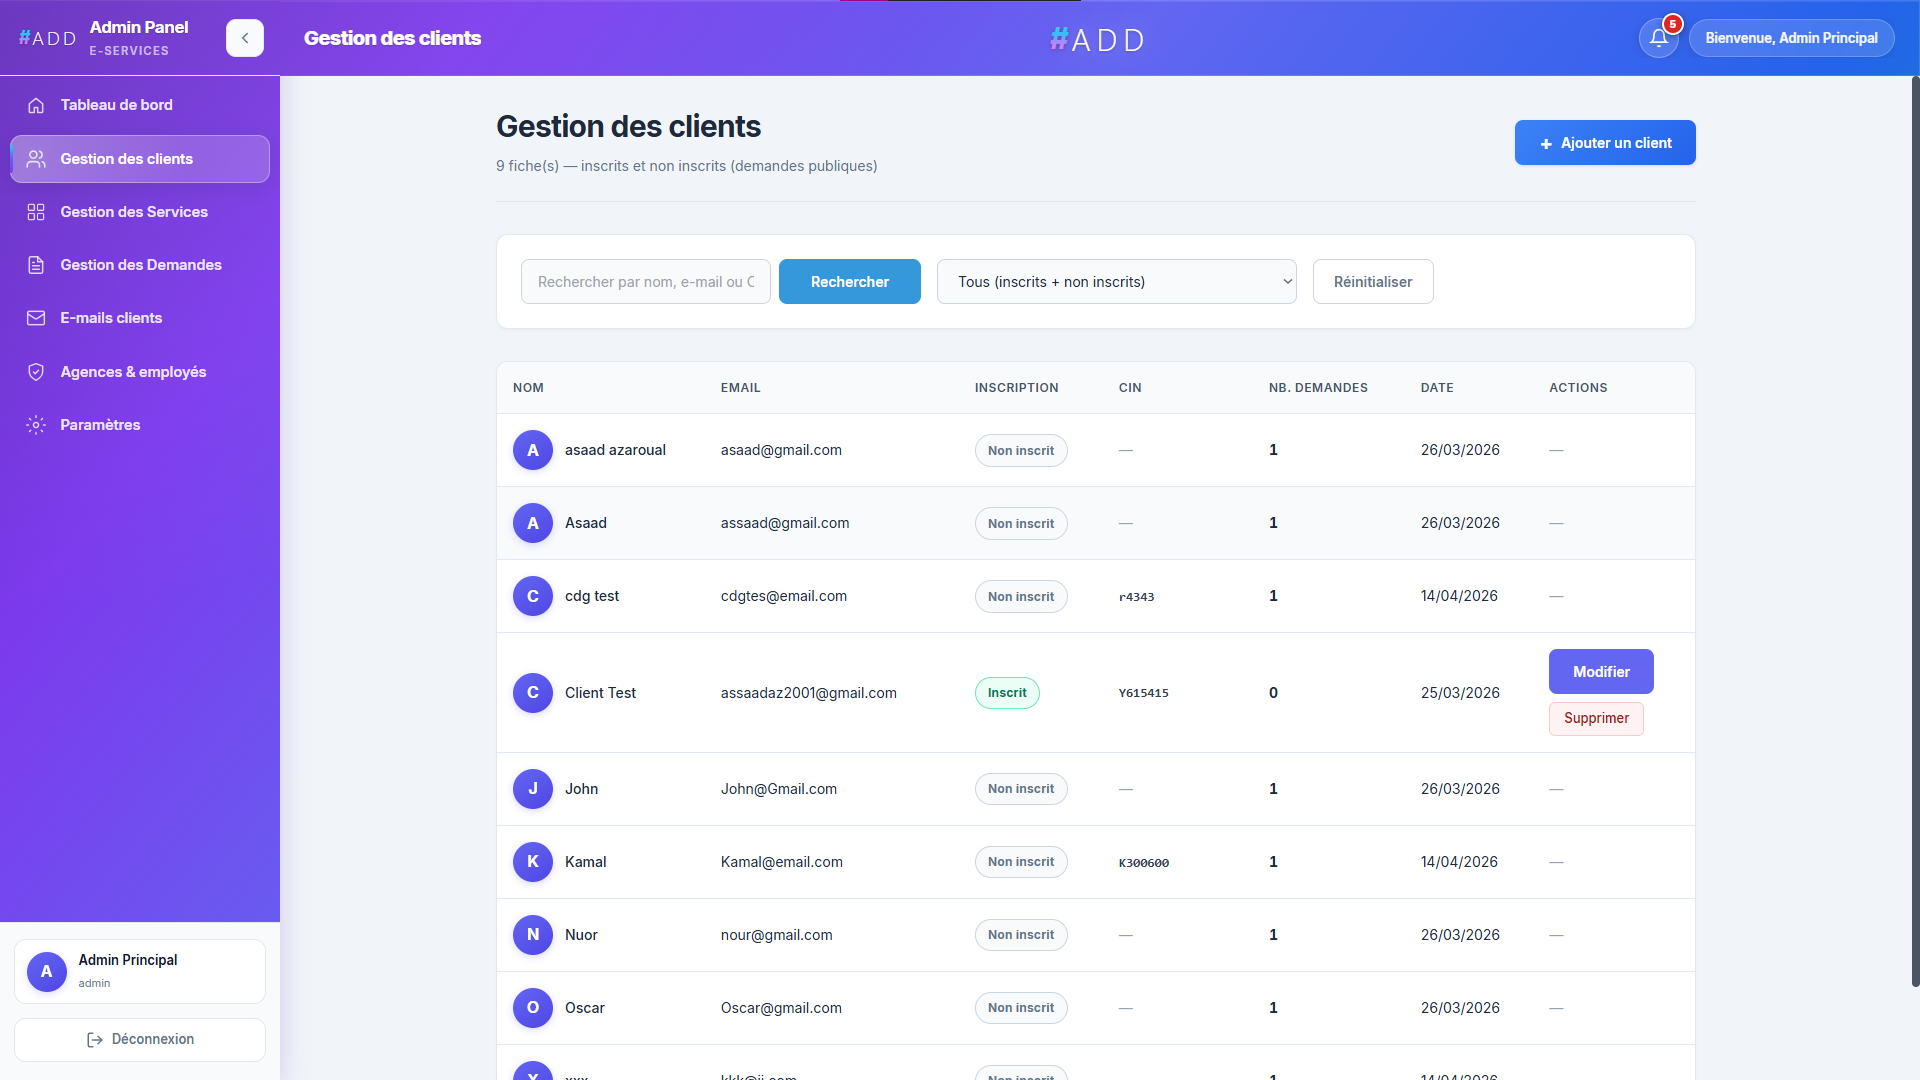
\includegraphics[width=0.95\textwidth]{admin-clients-list.png}
\caption{Interface de consultation de la liste des clients.}
\label{fig:admin-clients-list}
\end{figure}

La figure~\ref{fig:admin-clients-list} présente la liste des clients inscrits sur la plateforme. Cette interface facilite le suivi des comptes utilisateurs et permet à l'administrateur d'accéder rapidement aux informations essentielles relatives aux usagers.

\begin{figure}[H]
\centering
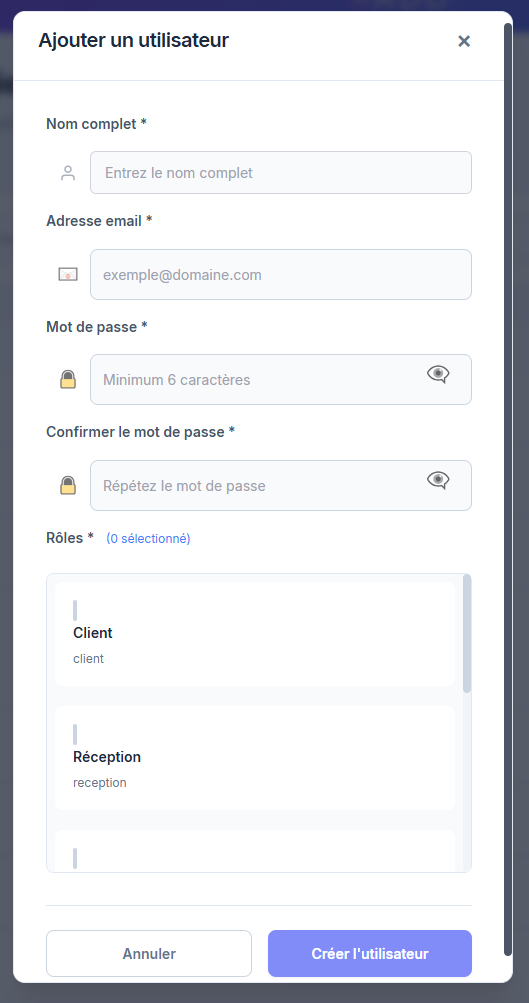
\includegraphics[width=0.7\textwidth]{admin-client-add.png}
\caption{Interface d'ajout d'un nouveau client.}
\label{fig:admin-client-add}
\end{figure}

La figure~\ref{fig:admin-client-add} illustre le formulaire d'ajout d'un nouveau client. L'administrateur peut y saisir les informations nécessaires à la création du compte utilisateur, ce qui permet d'assurer une gestion centralisée des usagers.

\newpage
\subsection{Gestion des agences}

Le module de gestion des agences permet d'administrer les entités institutionnelles participant à la plateforme. Chaque agence peut être associée à des services et à des employés.

\begin{figure}[H]
\centering
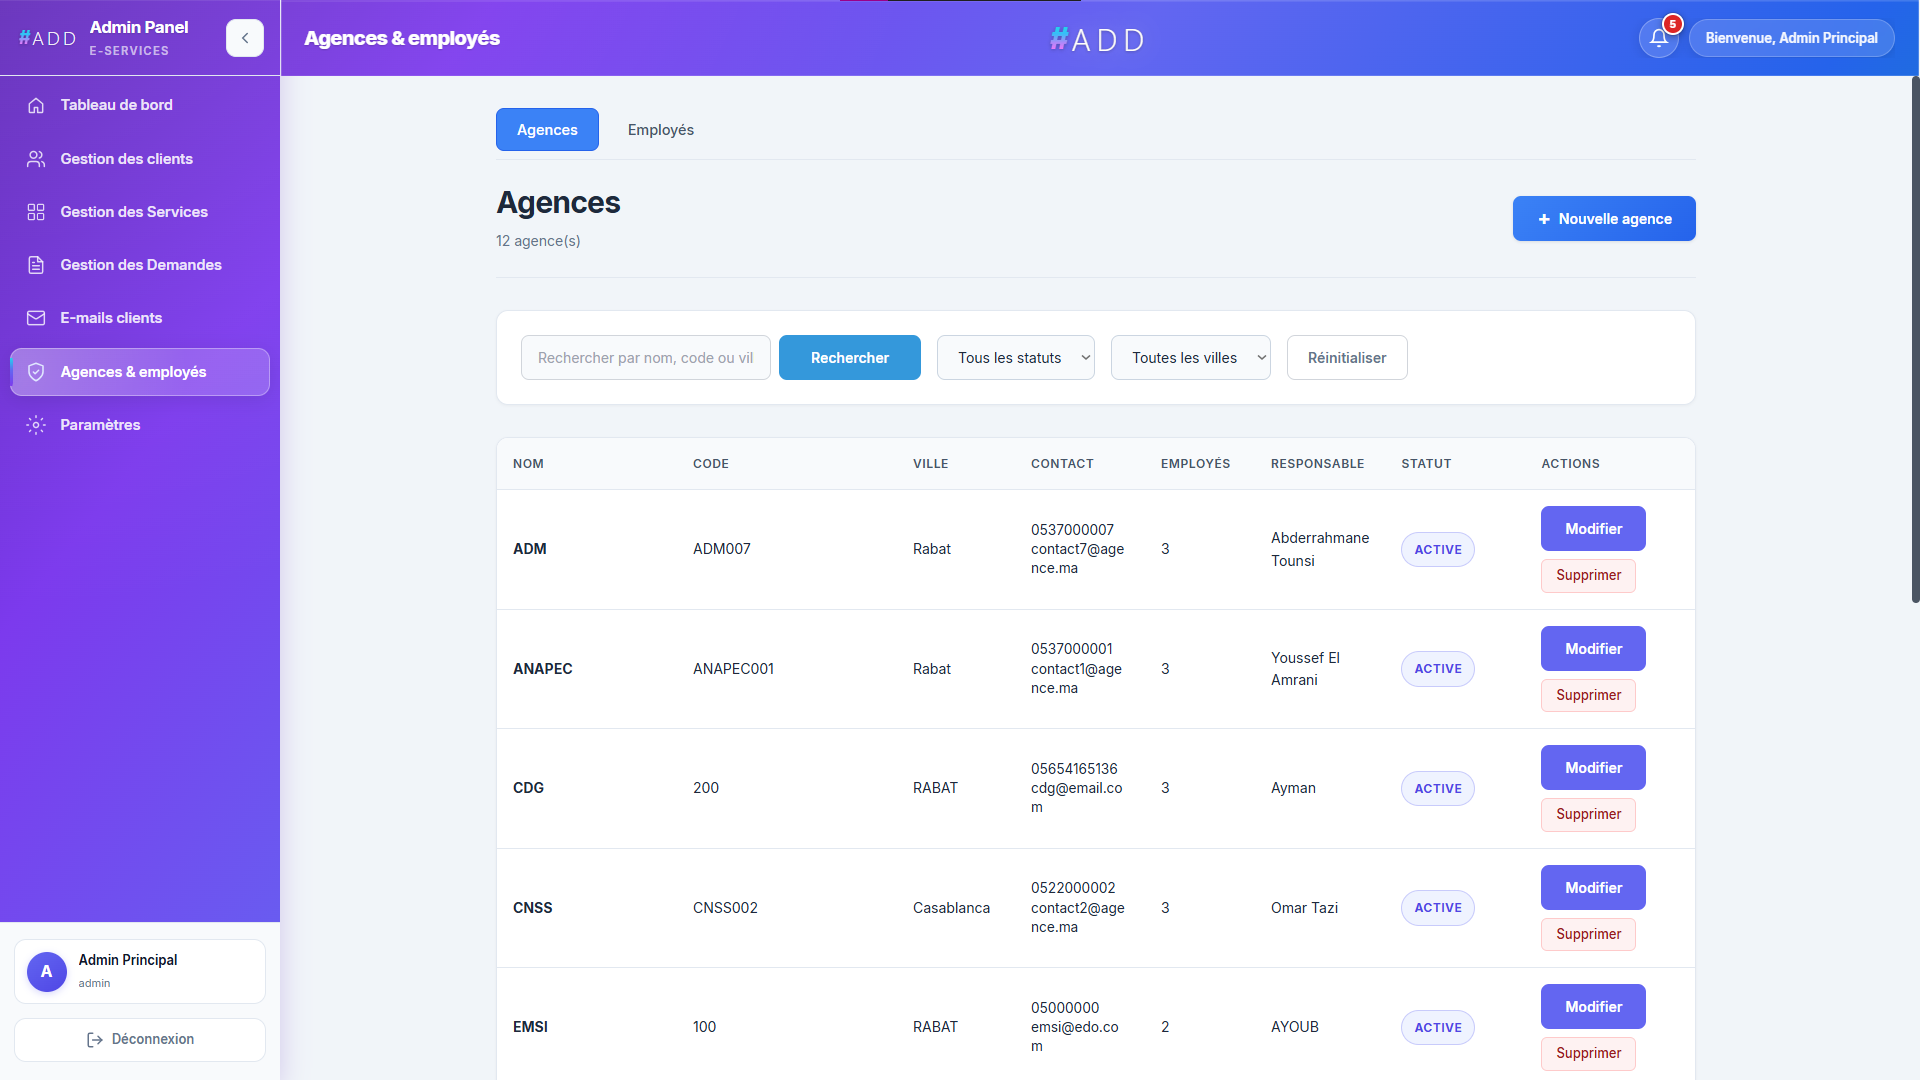
\includegraphics[width=0.95\textwidth]{admin-agencies-list.png}
\caption{Interface de consultation de la liste des agences.}
\label{fig:admin-agencies-list}
\end{figure}

La figure~\ref{fig:admin-agencies-list} présente la liste des agences enregistrées dans le système. Cette interface permet de consulter les informations principales de chaque agence et d'accéder aux actions de modification ou de gestion.

\begin{figure}[H]
\centering
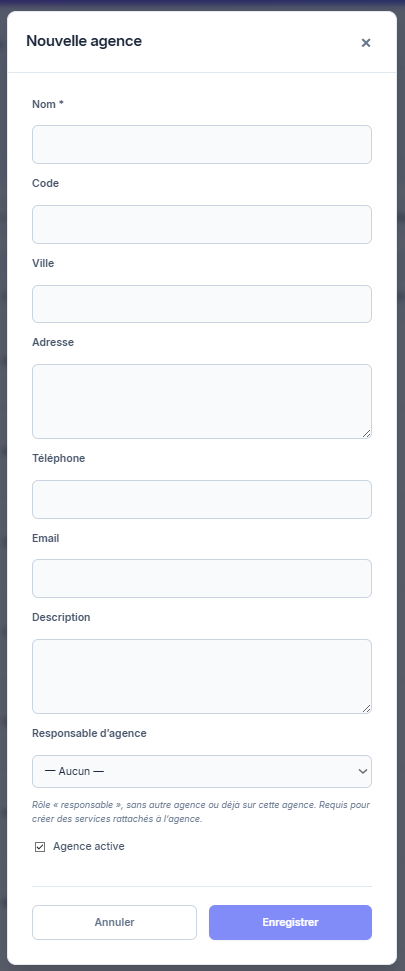
\includegraphics[width=0.5\textwidth]{admin-agency-add.png}
\caption{Interface d'ajout d'une nouvelle agence.}
\label{fig:admin-agency-add}
\end{figure}

La figure~\ref{fig:admin-agency-add} illustre le formulaire d'ajout d'une nouvelle agence. Cette fonctionnalité permet à l'administrateur d'enregistrer une nouvelle entité avec ses informations principales, afin de l'intégrer au processus de gestion des services et des demandes.

\newpage
\subsection{Gestion des employés}

Le module de gestion des employés permet d'administrer les comptes internes de la plateforme, notamment les agents, responsables et autres profils opérationnels. Chaque employé peut être associé à une agence et disposer d'un rôle adapté à ses responsabilités.

\begin{figure}[H]
\centering
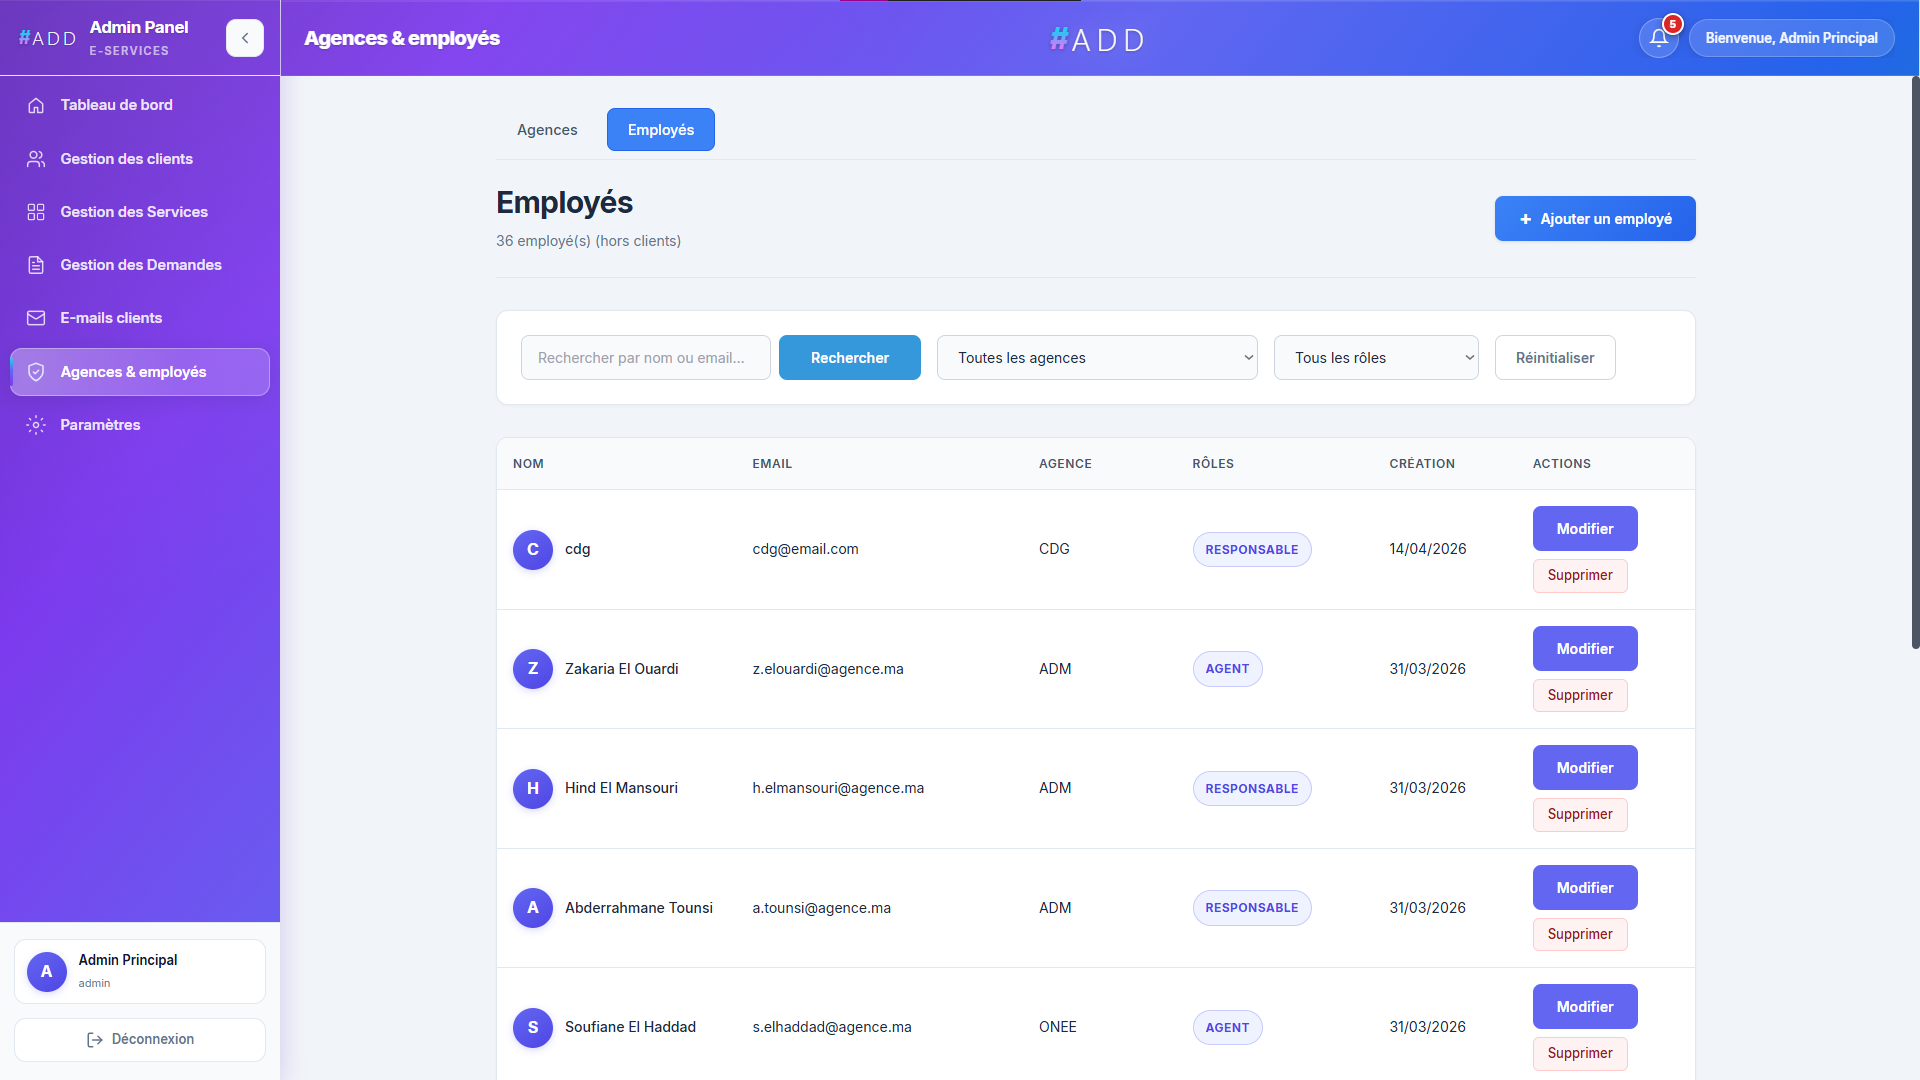
\includegraphics[width=0.95\textwidth]{admin-employees-list.png}
\caption{Interface de consultation de la liste des employés.}
\label{fig:admin-employees-list}
\end{figure}

La figure~\ref{fig:admin-employees-list} présente la liste des employés enregistrés dans le back-office. Cette interface facilite le suivi des comptes internes, de leurs rôles et de leur rattachement aux agences.

\begin{figure}[H]
\centering
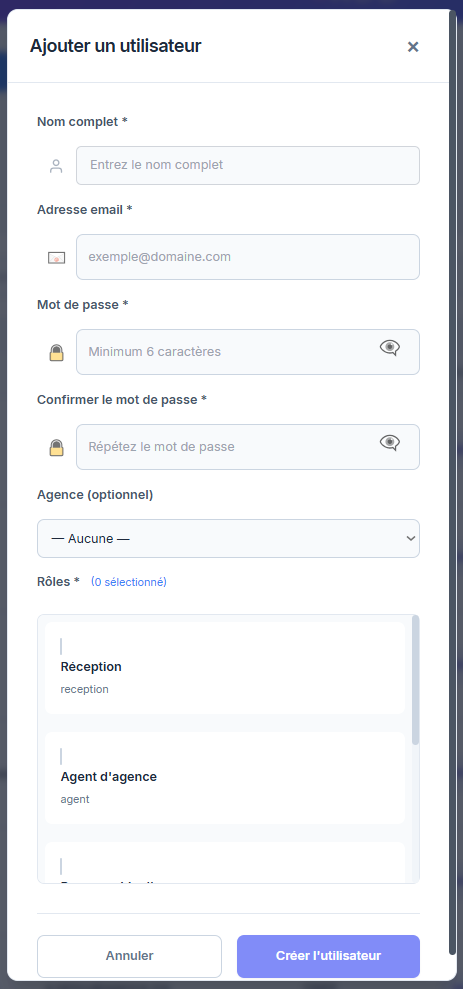
\includegraphics[width=0.6\textwidth]{admin-employee-add.png}
\caption{Interface d'ajout d'un nouvel employé.}
\label{fig:admin-employee-add}
\end{figure}

La figure~\ref{fig:admin-employee-add} illustre le formulaire d'ajout d'un nouvel employé. L'administrateur peut renseigner les informations personnelles, le rôle et l'agence de rattachement afin de créer un compte opérationnel conforme à l'organisation interne.

\newpage
\subsection{E-mails clients}

Le module des e-mails clients permet d'assurer la communication avec les usagers depuis le back-office. Il complète le système de notifications automatiques en offrant une interface dédiée aux échanges administratifs.

\begin{figure}[H]
\centering
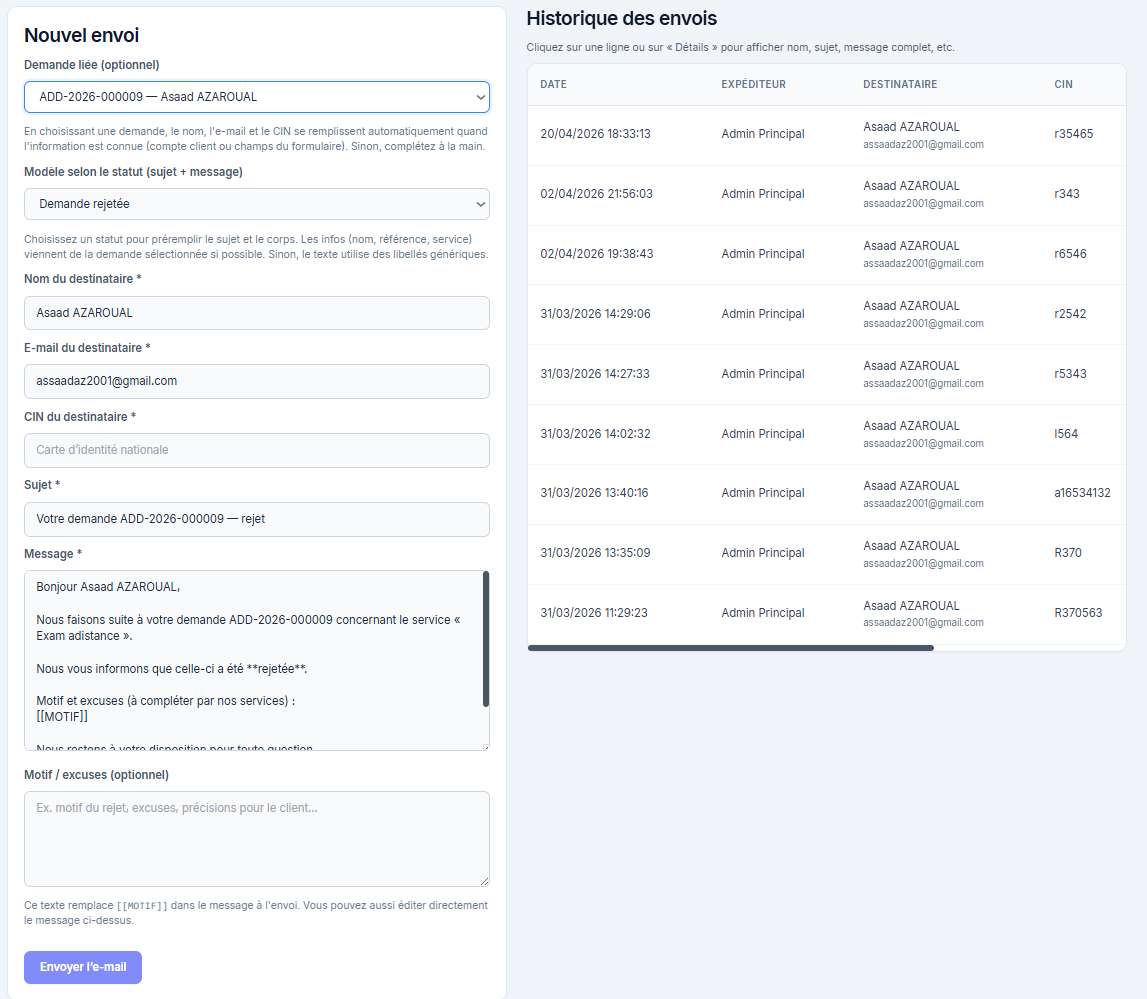
\includegraphics[width=1\textwidth]{admin-client-emails.png}
\caption{Interface de gestion des e-mails clients.}
\label{fig:admin-client-emails}
\end{figure}

La figure~\ref{fig:admin-client-emails} présente l'interface dédiée aux e-mails clients. Elle permet de centraliser les échanges avec les usagers et d'améliorer le suivi des communications liées aux demandes.

\newpage
\subsection{Notifications internes}

Les notifications internes permettent d'améliorer la réactivité des utilisateurs du back-office face aux nouvelles demandes soumises. Elles complètent les notifications envoyées par e-mail en offrant une alerte visuelle directement intégrée à l'interface.

\begin{figure}[H]
\centering

\includegraphics[width=0.15\textwidth]{notification-badge.png}
\caption{Badge de notification indiquant les demandes soumises non encore consultées.}
\label{fig:notification-badge}
\end{figure}

La figure~\ref{fig:notification-badge} montre le badge de notification intégré à l'en-tête du portail administratif. Le compteur indique le nombre de demandes soumises qui n'ont pas encore été consultées par un membre du personnel.

\begin{figure}[H]
\centering
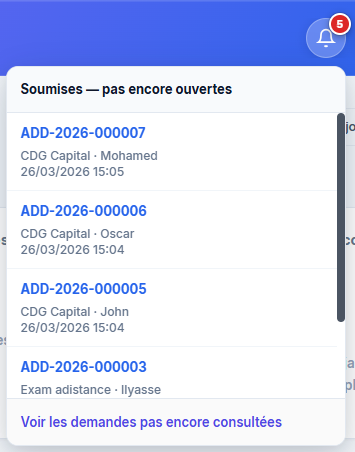
\includegraphics[width=0.4\textwidth]{notification-panel.png}
\caption{Panneau déroulant des notifications de demandes.}
\label{fig:notification-panel}
\end{figure}

La figure~\ref{fig:notification-panel} présente le panneau déroulant associé à l'icône de notification. Chaque entrée affiche les informations essentielles d'une demande, notamment sa référence, l'agence concernée, le demandeur et la date de soumission. Ce composant permet à l'administrateur ou à l'agent d'accéder rapidement aux nouvelles demandes sans quitter son contexte de travail.

\subsection{Paramètres utilisateur}

Le module des paramètres permet à l'utilisateur connecté de consulter et de modifier les informations liées à son profil. Cette fonctionnalité contribue à la personnalisation du compte et à la maintenance des données utilisateur.

\begin{figure}[H]
\centering
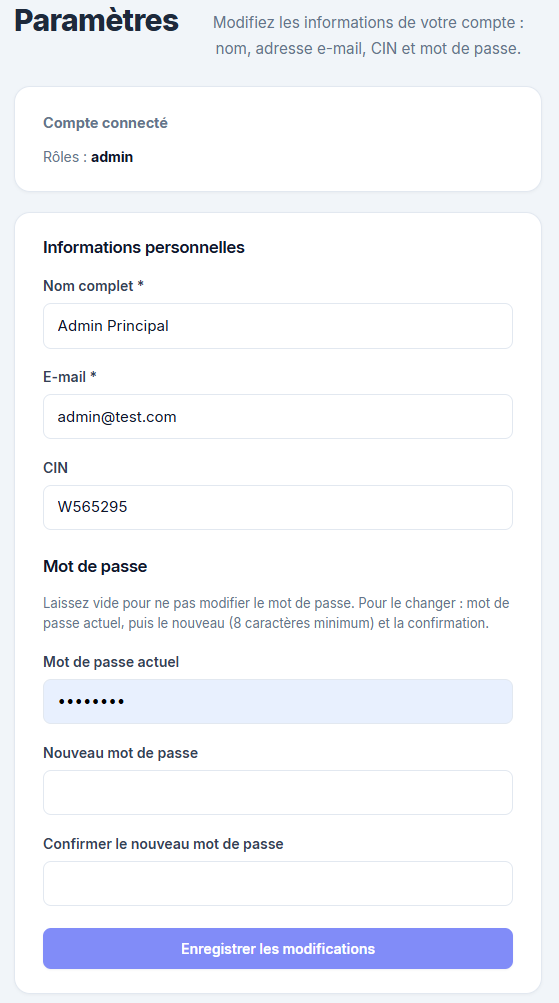
\includegraphics[width=0.6\textwidth]{admin-settings.png}
\caption{Interface de paramétrage du profil utilisateur.}
\label{fig:admin-settings}
\end{figure}

La figure~\ref{fig:admin-settings} présente l'écran des paramètres utilisateur. Cette interface permet la mise à jour des informations personnelles et contribue à la gestion autonome du profil.
```


\section{Interopérabilité et formats}

Les réponses d'erreur Laravel sont normalisées en JSON (messages de validation, codes HTTP). Les dates sont sérialisées en ISO-8601 côté API. La référence métier \texttt{ADD-AAAA-NNNNNN} est générée côté serveur pour les demandes \cite{owasp2021}.

\section{Journalisation et observabilité}

Laravel journalise via le canal configuré (\texttt{storage/logs/laravel.log} en développement). Les services métiers critiques (notifications) journalisent les succès et échecs d'envoi pour faciliter le diagnostic.

\section{Gestion des erreurs et robustesse}

Les contrôleurs s'appuient sur les exceptions HTTP de Laravel et sur les réponses structurées des Form Requests. Les transitions d'état vérifient le graphe autorisé avant persistance.

\section{Conclusion du chapitre}

L'implémentation décrite correspond au dépôt réalisé durant le stage : une API Laravel authentifiée par session Sanctum, un frontend React/Vite, une base PostgreSQL structurée par migrations, et des modules métiers (services dynamiques, demandes, agences, notifications). Le chapitre suivant présente les tests et la validation \cite{ieee1012,sommerville2016}.
